\section{Back-face Culling and Texture Mapping}

To texture our wireframe model, we first calculate the homography between the texture (2D image) and a face of the cube as it is projected in the 2D final image. We then use this homography to perspective warp the texture into the final image. See Figure \ref{subfig:texture}. But this is obviously not right, some faces overlap others randomly. We solve this by a technique called back-face culling.

Back-face culling is a technique we've employed to address the problem that appears when we render the whole cube. In the 2D view you can not see all 5 textured faces of the cube at once. It is only possible to see one to three faces at any given time. Therefore some faces we render are redundant. All faces are drawn in the order in which the list containing their names is processed, so it is the same order always. Therefore the faces that are drawn later occlude faces drawn earlier, even though logically they should be behind them. 

To address this problem, a simple technique has been developed, where we determine the angle between the camera and a face, and based on that we decide whether or not to show the face. First we compute the unitary normal vector of the face. We take three points from the face, since we assume that the face is composed of four coplanar points, it does not matter which three we take, but the order does matter, because with wrong order we will get a normal that faces the other way (inside the cube). We then construct displacement vectors between two point pairs of the three points, and calculate the cross product of these vectors. As the last step we transform the obtained vector to get a unitary vector. 

Similarly we compute a vector from camera center and the center of the face we are comparing. We transform this vector to unitary as well. We can calculate the angle between the two vectors. If this angle is greater than 90 degrees, we know that the face is facing away from the camera, and we therefore don't draw it.

 \begin{figure}[h!]
	\begin{subfigure}[b]{0.5\textwidth}
		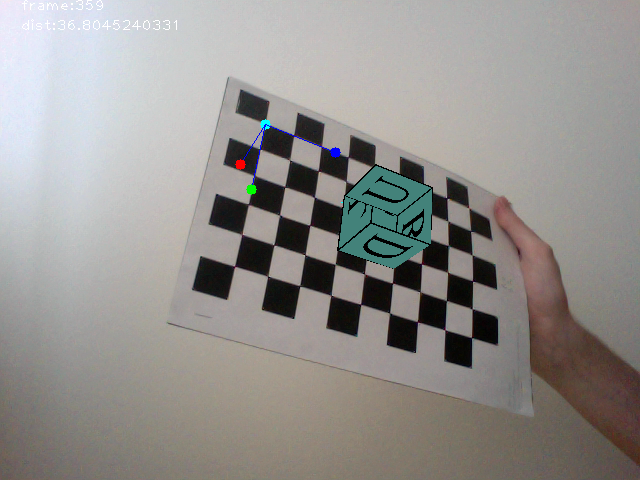
\includegraphics[width=\textwidth]{Handin3/images/culling.png}
		\caption{Texture Mapping}
		\label{subfig:texture}
	\end{subfigure}
	~
	\begin{subfigure}[b]{0.5\textwidth}
		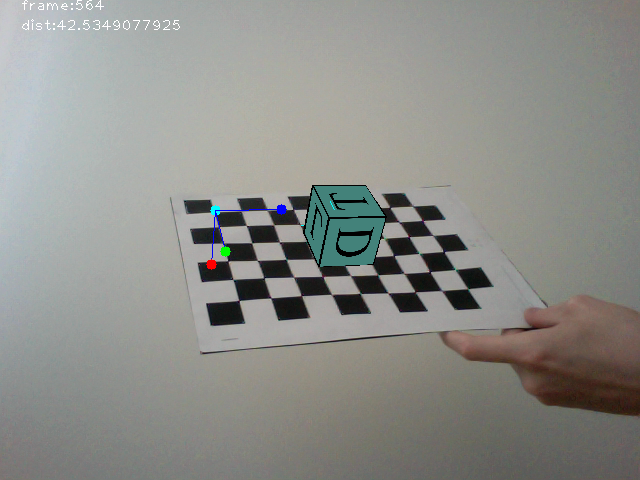
\includegraphics[width=\textwidth]{Handin3/images/texture2.png}
		\caption{Back-face Culling}
		\label{subfig:backculling}
	\end{subfigure}
	
	\label{fig:texturing}
	\caption{Backface Culling and Texture Mapping}
\end{figure}